\chapter{Apache Kafka nel settore dell’Integrazione Aziendale}

\section{L'evoluzione delle architetture di integrazione}
Per soddisfare le richieste clientelari ed essere sempre competitiva e all'avanguardia, una priorità aziendale sono le esplorazioni tecnologiche e di prodotto anche tramite l'utilizzo di percorsi di \textit{stage} insieme ai laureandi, come quanto accaduto nella mia esperienza.

% Introduzione al motivo aziendale per cui è nato questo percorso di stage: la propensione odierna alle architetture a microservizi, la gestione di grandi flussi di dati in modo efficiente ed eff1icace, una richiesta di un sistema innovativo da parte della clientela.3
Nel settore dell'\textit{Enterprise Application Integration} in particolare, l'evoluzione tecnologica è diretta verso soluzioni sempre più distribuite e con un flusso di dati in continuo aumento.
Uno degli obiettivi specifici dell'area EAI di Sync Lab è pertanto quello di trovare un software o tecnologia in grado di soddisfare i bisogni dei clienti di gestire un flusso di dati di dimensioni molto maggiori a quelle attuali, tramite architetture a messaggio che utilizzano servizi distribuiti.

% \section{L’evoluzione delle architetture di integrazione}
%
% % Introduzione al motivo aziendale per cui è nato questo percorso di stage: la propensione odierna alle architetture a microservizi, la gestione di grandi flussi di dati in modo efficiente ed eff1icace, una richiesta di un sistema innovativo da parte della clientela.3
% L'evoluzione del settore dell'\textit{Enterprise Application Integration} verso soluzioni sempre più distribuite e con un flusso di dati in continuo aumento ha sviluppato nei clienti (e di conseguenza nell'azienda) un interesse verso il prodotto Apache Kafka.
% Il software ha dimostrato negli anni recenti un notevole successo in diversi campi; l'azienda ha interesse nel testare le capacità di Kafka nel soddisfare le esigenze dell'integrazione aziendale.
%
% \bigskip
% \begin{figure}[h]
%   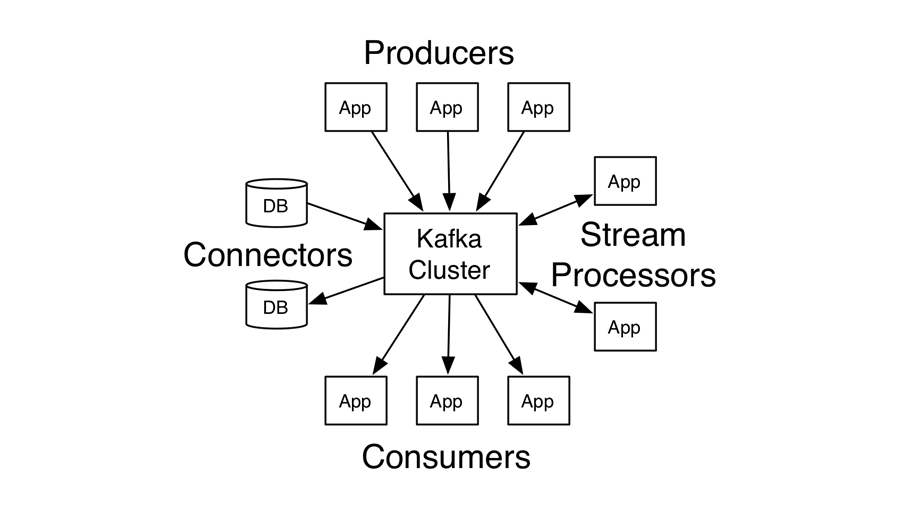
\includegraphics[width=\textwidth]{images/kafka.png}\\
%   \caption{Illustrazione di un sistema a servizi con Apache Kafka}
%   \captionsetup{aboveskip=2pt,font=it}
%   \caption*{Fonte: https://kafka.apache.org/20/documentation.html}
% \end{figure}
%
% Kafka è una piattaforma di \textit{event streaming}, un sistema moderno e distribuito basato sugli eventi anzichè su di una soluzione più classica come può essere quella del \textit{request/response}.
% L'adozione del \textit{software} nell'ambito dell'EAI è in crescita dato le dimostrate qualità nel gestire grandi moli di dati: la sua performance, sicurezza e scalabilità sono i punti che hanno portato il software al suo attuale successo.
%
% % \bigskip\noindent
% % Esposizioni delle ragioni personali che hanno portato alla scelta di tale percorso.


\section{Apache Kafka come Middleware}

Per soddisfare le esigenze di innovazione l'azienda ha avviato un percorso per indagare le capacità del software Apache Kafka nell'ambito dell'integrazione aziendale.

\bigskip
\begin{figure}[h]
  \begin{center}
    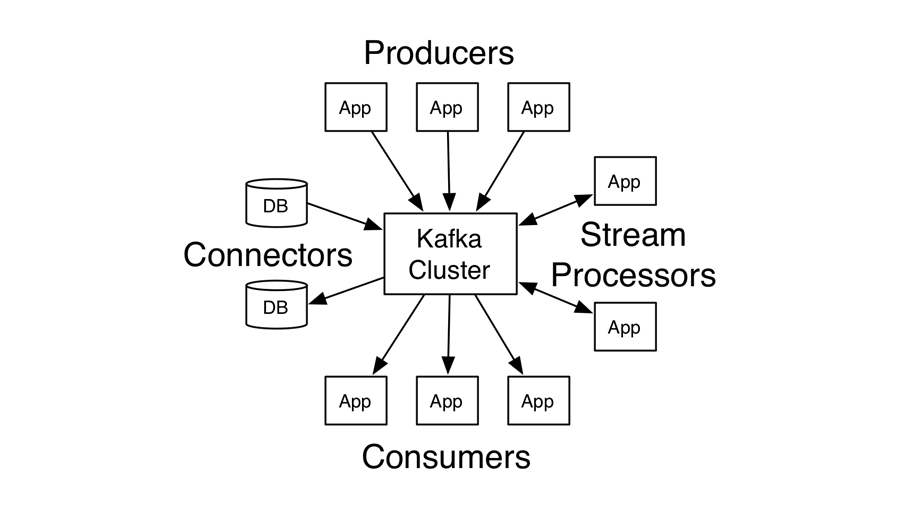
\includegraphics[width=0.8\textwidth]{images/kafka.png}\\
    \caption{Illustrazione di un sistema a servizi con Apache Kafka}
    \captionsetup{aboveskip=2pt,font=it}
    \caption*{Fonte: https://kafka.apache.org/20/documentation.html}
  \end{center}
\end{figure}

Kafka è una piattaforma di \textit{event streaming}, un sistema moderno e distribuito basato sugli eventi anzichè su di una soluzione più classica come può essere quella del \textit{request/response}.
Apache Kafka si integra ottimamente in molti sistemi basati sulle Architetture a messaggio, in cui lo scambio affidabile di dati in tempo reale è la priorità.

Il software ha dimostrato negli anni recenti un notevole successo in diversi campi, come quello del flusso di \textit{Big Data}, del monitoraggio e dell'elaborazione dati in tempo reale.
L'adozione del \textit{software} nell'ambito dell'EAI è in crescita dato le dimostrate qualità nel gestire grandi moli di dati: la sua performance, sicurezza e scalabilità sono i punti che hanno portato il software al suo attuale successo.

L'interesse di Sync Lab nel \textit{software} risiede dunque nell'utilizzo di Kafka come un  \textit{Middleware} per soddisfare i problemi di integrazione aziendale e reingegnerizzare i flussi di dati preesistenti, ovvero sviluppare un nuovo sistema che consenta la comunicazione tra differenti servizi con un rapido flusso di dati fra di essi.
L'azienda ha avviato un percorso per testare le capacità di Kafka rispetto agli attuali strumenti utilizzati nel settore, per valutare i vantaggi e svantaggi che l'adozione di tale software può fornire al cliente.

\bigskip\noindent
Sono numerosi i vantaggi che Kafka può portare nel settore, fra cui:
\begin{itemize}
  \item gestione rapida e performante di un enorme flusso di dati;
  \item scalabilità;
  \item sicurezza riguardo la persistenza dei dati;
  \item semplice integrazione e affiancamento a sistemi già esistenti;
  \item l'essere una piattaforma \textit{open source};
  \item processazione dei dati in tempo reale integrata.
\end{itemize}

% \bigskip\noindent
% TODO: Come Kafka possa risolvere i problemi e le necessità viste qui sopra.

\section{Il percorso di Stage}


% Descrizione di come il percorso di \textit{stage} si inserisce nella visione più ampia riportata qui sopra.
%
% \bigskip\noindent
% Elenco degli obiettivi del percorso:
% \begin{itemize}
%   \item formazione riguardo Kafka e l’ambito dell’integrazione;
%   \item verificare le capacità di Kafka nell’ambito EAI;
%   \item sperimentare l’utilizzo di Kafka come \textit{Middleware} tramite una simulazione di un caso d’uso reale a servizi indipendenti.
% \end{itemize}
%
% \noindent
% Breve esposizione dei motivi che mi hanno portato a scegliere questo percorso

% TODO:
% - motivazioni riguardo il percorso di stage proposto
% - descrizione del percorso di stage tenendo conto del contesto e degli obiettivi citati sopra
% - descrivere i miei obiettivi rispetto a quelli aziendali
Il percorso di \textit{stage} offerto dall'azienda si inserisce all'interno della strategia aziendale più ampia descritta qui sopra.
Al fine di esplorare la tecnologia di Apache Kafka nell'ambito di un \textit{Middleware} per l'integrazione aziendale, l'azienda ha proposto un percorso di stage il cui obiettivo è la reingegnerizzazione di un flusso di dati asincrono, utilizzando un'architettura basata su Kafka all'interno di un caso d'uso simulato tramite servizi indipendenti.
Lo stagista ha il compito di osservare, testare e verificare che il \textit{software} possa svolgere alcuni compiti inerenti all'area dell'EAI, analizzando alcuni casi d'uso presenti in un \textit{Middleware} aziendale in ambito \textit{telco}.

\bigskip\noindent
Il percorso proposto prevede le seguenti attività e obiettivi generali:
\begin{itemize}
  \item formazione riguardo la piattaforma di \textit{event streaming} Kafka e l'ambito dell'integrazione aziendale;
  \item verifica delle capacità di Kafka nell'EAI;
  \item sperimentazione e sviluppo di un \textit{Middleware} basato su Kafka tramite una simulazione di un caso d'uso reale a servizi indipendenti.
\end{itemize}

\bigskip\noindent
I prodotti attesi al termine dello \textit{stage} sono dunque associati alla realizzazione di tre flussi di integrazione, basati su dei casi d’uso reali, per la gestione dei paradigmi di integrazione asincrono e asincrono con Callback (due requisiti obbligatori), e sincrono ove fosse disponibile del tempo aggiuntivo e se ritenuto opportuno; durante il percorso considerato il contesto e le opportunità offerte dal \textit{software} questo obiettivo verrà sostituito per testare delle funzionalità aggiuntive di Kafka.

La realizzazione di questi prodotti necessita una sostanziale formazione dello stagista riguardo i principali concetti del settore del \textit{Enterprise Application Integration} e l'utilizzo della piattaforma di \textit{event streaming} Kafka.
Più precisamente, i contenuti formativi previsti durante questo percorso di \textit{stage} sono i seguenti:
\begin{itemize}
  \item Concetti chiave di Enterprise Application Integration
  \item Design archittetturali
  \item Cenni di Networking applicato alle architetture distribuite
  \item Architetture di Integrazione e Middleware
  \item Apache Kafka
\end{itemize}


\section{Motivazioni e obiettivi personali}

La ragione principale che mi ha portato a scegliere questo percorso di \textit{stage} è l'interesse verso Apache Kafka, la cui formazione ritengo possa arricchire fortemente le mie capacità professionali.
L'utilizzo della piattaforma di \textit{event streaming} è sempre più in crescita, come l'evoluzione verso sistemi sempre più distribuiti e a microservizi
Sono pertanto interessato a sviluppare la mia formazione riguardo l'utilizzo e le implicazioni di questa tecnologia in rapida espansione, la cui formazione potrà essermi utile in molti campi anche al di fuori degli obiettivi dell'azienda ospitante lo \textit{stage}
Altri fattori fondamentali alla scelta del percorso sono stati la famigliarità con l'azienda, il personale giudizio positivo che ho avuto riguardo il loro metodo di lavoro e la libertà di sviluppo concessa: ho ritenuto importante la possibilità di elaborare personalmente un'architettura del caso d'uso con una visione ad alto livello, anzichè il semplice sviluppo di un software predeterminato e dal percorso strettamente imposto.
